\pdfminorversion=4
\documentclass[compress,
mathserif,wide,%red,
%handout
]{beamer}

\usepackage{amsmath,amsfonts,bm,bbm,comment}
\usepackage{latexsym,tabularx,amscd}
\usepackage{etex} 
\usepackage{algorithm}
\usepackage[noend]{algorithmic}
\usepackage{subfigure}
\usepackage{url}
%\usepackage{multimedia}
\usepackage{hyperref}
\usepackage{skull}
%\usepackage{enumitem}
%\usepackage{movie15}

\usepackage{multirow}
\usepackage{cancel}

%\usepackage{ulem}
\usepackage{lmodern}
\usepackage{array} 
\usepackage{etoolbox}
\usepackage{caption}
\usepackage[normalem]{ulem}

\usepackage{mathtools}

\usepackage[space]{grffile}

\usepackage{tikz}
\usetikzlibrary{shapes.arrows}
\usetikzlibrary{arrows,positioning}
\usepackage{pgfplots}
%\usetikzlibrary{pgfplots.groupplots}

\tikzset{
    myarrow/.style={
        draw,
        fill=black,
        single arrow,
        minimum height=6ex,
        single arrow head extend=1ex
    }
}


\newcommand{\vertiii}[1]{{\left\vert\kern-0.25ex\left\vert\kern-0.25ex\left\vert #1 
    \right\vert\kern-0.25ex\right\vert\kern-0.25ex\right\vert}}

\newcommand{\vertiiibig}[1]{{\big\vert\kern-0.25ex\big\vert\kern-0.25ex\big\vert #1 
    \big\vert\kern-0.25ex\big\vert\kern-0.25ex\big\vert}}

\newcommand{\vertiiiplain}[1]{{\vert\kern-0.25ex\vert\kern-0.25ex\vert #1 
    \vert\kern-0.25ex\vert\kern-0.25ex\vert}}



\usepackage{dsfont}
\DeclareMathOperator{\ind}{\mathds{1}}  % Indicator


\newcommand{\abs}[1]{\left|#1\right|}

\mode<presentation>

\usetheme{Madrid}
% other themes: AnnArbor, Antibes, Bergen, Berkeley, Berlin, Boadilla,
% boxes, CambridgeUS, Copenhagen, Darmstadt, default, Dresden,
% Frankfurt, Goettingen, Hannover, Ilmenau, JuanLesPins, Luebeck,
% Madrid, Maloe, Marburg, Montpellier, PaloAlto, Pittsburg, Rochester,
% Singapore, Szeged, classic

% \usecolortheme{lily} 
% color themes: albatross, beaver, beetle, crane, default, dolphin,
% dov, fly, lily, orchid, rose, seagull, seahorse, sidebartab,
% structure, whale, wolverine

% \usefonttheme{serif} 
% font themes: default, professionalfonts, serif, structurebold,
% structureitalicserif, structuresmallcapsserif

%\usefonttheme[onlymath]{serif}
%\usefonttheme[onlylarge]{structuresmallcapsserif} 
  
%\useoutertheme[subsection=false]{smoothbars}
% outer themes:
% default,infolines,miniframes,smoothbars,sidebar,split,shadow,tree,smoothtree
%\useinnertheme{rectangles}
\beamertemplatenavigationsymbolsempty

% \definecolor{fore}{RGB}{249,242,215}
% \definecolor{back}{RGB}{51,51,51}
% \definecolor{title}{RGB}{255,0,90}
% \setbeamercolor{titlelike}{fg=title}
% \setbeamercolor{normal text}{fg=fore,bg=back}
% \setbeamercovered{transparent}
  % or whatever (possibly just delete it)
%\beamertemplatenavigationsymbolsempty

\usepackage[english]{babel}
\usepackage[latin1]{inputenc}
% or whatever
%\usepackage{comicsans} 
%\renewcommand{\sfdefault}{comic} 
%\usepackage{mathptmx}
%\mathversion{bold}
%\usepackage{helvet}
%\usepackage{courier}

%\usepackage[T1]{fontenc}
% Or whatever. Note that the encoding and the font should match. If T1
% does not look nice, try deleting the line with the fontenc.


%%%% Figures %%%%%


\newcommand{\LectureFigs}{../Figures}


\definecolor{bluegray}{rgb}{0.15,0.20,0.40}
\definecolor{bluegraylight}{rgb}{0.35,0.40,0.60}
\definecolor{gray}{rgb}{0.3,0.3,0.3}
\definecolor{lightgray}{rgb}{0.7,0.7,0.7}
\definecolor{brightblue}{rgb}{0.1,0.4,0.7}
\definecolor{darkblue}{rgb}{0.1,0.1,0.6}
\definecolor{darkgreen}{rgb}{0.0,0.5,0.2}
\definecolor{orange}{rgb}{0.7,0.3,0}

\def \captioncolor { }

\setbeamertemplate{itemize item}{{\color{black}$\bullet$}}
\setbeamertemplate{itemize subitem}{{\color{black}$\circ$}}
\setbeamertemplate{frametitle}[default][center]
\setbeamerfont{frametitle}{series=\bfseries}
\addtobeamertemplate{frametitle}{\vskip1ex}{ \vspace{0.5em} \hrule}
\setbeamercolor{frametitle}{fg=,bg=}

\setbeamertemplate{theorems}[numbered]
\setbeamertemplate{caption}[numbered]
\setbeamertemplate{algorithm}[numbered]

\numberwithin{theorem}{subsection}
\numberwithin{equation}{subsection}
\numberwithin{figure}{subsection}
\numberwithin{algorithm}{subsection}


%\setbeamerfont{page number in head/foot}{size=\scriptsize}
\setbeamertemplate{footline}[frame number]
\setbeamercolor{page number in head/foot}{fg=black}
\setbeamersize{text margin left=2em,text margin right=2em}

\setbeamertemplate{footline}
{
    %\hspace{3em} \insertshorttitle \hfill \insertframenumber / \inserttotalframenumber\hspace{3em}
    \hspace{3em} \insertshorttitle \hfill \insertsubsectionnumber-\insertframenumber \hspace{3em}
    \vspace{1.5em}
}

\definecolor{babyblueeyes}{rgb}{0.63, 0.79, 0.95}
\definecolor{bleudefrance}{rgb}{0.19, 0.55, 0.91}
\definecolor{matlabPlotBlue}{rgb}{0.25, 0.58, 0.8}
\definecolor{matlabPlotOrange}{rgb}{0.855, 0.324, 0.098}



\captionsetup[figure]{labelfont={color=black}}

\AtBeginEnvironment{lemma}{%
  \setbeamercolor{block title}{fg=black,bg=babyblueeyes}
  \setbeamercolor{block body}{fg=black,bg=}
  \setbeamerfont*{block title}{series=\bfseries}
}

\AtBeginEnvironment{theorem}{%
  \setbeamercolor{block title}{fg=black,bg=babyblueeyes}
  \setbeamercolor{block body}{fg=black,bg=}
  \setbeamerfont*{block title}{series=\bfseries}
}

\AtBeginEnvironment{corollary}{%
  \setbeamercolor{block title}{fg=black,bg=babyblueeyes}
  \setbeamercolor{block body}{fg=black,bg=}
  \setbeamerfont*{block title}{series=\bfseries}
}

\AtBeginEnvironment{fact}{%
  \setbeamercolor{block title}{fg=black,bg=babyblueeyes}
  \setbeamercolor{block body}{fg=black,bg=}
  \setbeamerfont*{block title}{series=\bfseries}
}

\AtBeginEnvironment{definition}{%
  \setbeamercolor{block title}{fg=black,bg=babyblueeyes}
  \setbeamercolor{block body}{fg=black,bg=}
  \setbeamerfont*{block title}{series=\bfseries}
}

\newenvironment<>{varblock}[2][.9\textwidth]{%
  \vspace{-1em}
  \begin{center}
  \begin{minipage}{#1}
  %\setlength{\textwidth}{#1}
  \begin{actionenv}#3%
    \def\insertblocktitle{#2}%
    \par%
    \usebeamertemplate{block begin}}
  {\par%
    \usebeamertemplate{block end}%
  \end{actionenv}
  \end{minipage}
  \end{center}
}


\newcommand\blankfootnote[1]{%
  \let\thefootnote\relax\footnotetext{#1}%
  \let\thefootnote\svthefootnote%
}


%%%%%
\newcommand{\bb}{\bm b}
\newcommand{\bZ}{\bm Z}
\newcommand{\bC}{\bm C}
\newcommand{\cU}{{\cal U}}
\newcommand{\bR}{{\bm R}}
\newcommand{\bi}{{\bm i}}
\newcommand{\bS}{{\bm S}}
\newcommand{\cE}{{\cal E}}
\newcommand{\cF}{{\cal F}}
\newcommand{\bk}{{\bm k}}
\newcommand{\bu}{{\bm u}}
\newcommand{\bx}{{\bm x}}
\newcommand{\bA}{{\bm A}}
\newcommand{\bh}{{\bm h}}
\newcommand{\by}{{\bm y}}
\newcommand{\bI}{{\bm I}}
\newcommand{\ba}{{\bm a}}
\newcommand{\bw}{{\bm w}}
\newcommand{\bPhi}{{\bm \Phi}}
\newcommand{\bX}{{\bm X}}
\newcommand{\bY}{{\bm Y}}
\newcommand{\bM}{{\bm M}}
\newcommand{\be}{{\bm e}}
\newcommand{\bs}{{\bm s}}
\newcommand{\bB}{{\bm B}}
\newcommand{\bW}{{\bm W}}
\newcommand{\bN}{{\bm N}}
\newcommand{\bU}{{\bm U}}
\newcommand{\bV}{{\bm V}}
\newcommand{\bP}{{\bm P}}
\newcommand{\bH}{{\bm H}}
\newcommand{\bSigma}{{\bm \Sigma}}
\newcommand{\bL}{{\bm L}}



\newcommand{\bv}{\bm v}
\newcommand{\eps}{\epsilon}
\newcommand{\vf}{\varphi}
\newcommand{\de}{\delta}
\newcommand{\<}{\langle}
\renewcommand{\>}{\rangle}
\newcommand{\goto}{\rightarrow}
\newcommand{\argmin}{\mbox{argmin}}
\newcommand{\argmax}{\mbox{argmax}}
\newcommand{\Ave}{\mathop{\rm Ave}\nolimits}
\newcommand{\sgn}{\mbox{sgn}}
\newcommand{\cN}{\mathcal{N}}
\newcommand{\cR}{\mathcal{R}}

\def\C{{\mathbb{C}}}
\def\R{{{\mathbb{R}}}} %seemed too large in subscripts, so I changed --JW 
\def\P{{\hbox{\bf P}}}
\def\Z{{{\mathbb{Z}}}}
\def\T{{\hbox{\bf T}}}


\newcommand{\cA}{\mathcal{A}}
\newcommand{\cP}{\mathcal{P}}
\newcommand{\cD}{\mathcal{D}}
\newcommand{\cL}{\mathcal{L}}
\newcommand{\shrink}{\text{shrink}}


\newcommand{\Obs}{\Omega_{\text{obs}}}


\renewcommand{\P}{\operatorname{\mathbb{P}}}
\newcommand{\E}{\operatorname{\mathbb{E}}}

% Linear algebra macros
%\newcommand{\vct}[1]{#1}
%\newcommand{\mtx}[1]{#1}
\newcommand{\vct}[1]{\bm{#1}}
\newcommand{\mtx}[1]{\bm{#1}}
%\newcommand{\mtx}[1]{\mathsfsl{#1}}

\newcommand{\transp}{T}
\newcommand{\adj}{*}
\newcommand{\psinv}{\dagger}
\newcommand{\lspan}[1]{\operatorname{span}{#1}}

\newcommand{\range}{\operatorname{range}}
\newcommand{\colspan}{\operatorname{colspan}}

\newcommand{\rank}{\text{rank}}

\newcommand{\diag}{\operatorname{diag}}
\newcommand{\trace}{\text{Tr}}

\newcommand{\supp}[1]{\operatorname{supp}(#1)}

\newcommand{\smax}{\sigma_{\max}}
\newcommand{\smin}{\sigma_{\min}}

\newcommand{\restrict}[1]{\big\vert_{#1}}

\newcommand{\Id}{\text{\em I}}
\newcommand{\OpId}{\mathcal{I}}



% define your own colors:
\definecolor{Red}{rgb}{1,0,0}
\definecolor{Blue}{rgb}{0,0,1}
\definecolor{Green}{rgb}{0,1,0}
\definecolor{magenta}{rgb}{1,0,.6}
\definecolor{lightblue}{rgb}{0,.5,1}
\definecolor{lightpurple}{rgb}{.6,.4,1}
\definecolor{gold}{rgb}{.6,.5,0}
\definecolor{orange}{rgb}{1,0.4,0}
\definecolor{hotpink}{rgb}{1,0,0.5}
\definecolor{newcolor2}{rgb}{.5,.3,.5}
\definecolor{newcolor}{rgb}{0,.3,1}
\definecolor{newcolor3}{rgb}{1,0,.35}
\definecolor{darkgreen1}{rgb}{0, .35, 0}
\definecolor{darkgreen}{rgb}{0, .6, 0}
\definecolor{darkred}{rgb}{.75,0,0}

\xdefinecolor{olive}{cmyk}{0.64,0,0.95,0.4}
\xdefinecolor{purpleish}{cmyk}{0.75,0.75,0,0}

\definecolor{lightgrey}{RGB}{186,186,186}
\definecolor{back}{RGB}{51,51,51}
\definecolor{fore}{RGB}{249,242,215}
\definecolor{back}{RGB}{51,51,51}
\definecolor{title}{RGB}{255,0,20}
\definecolor{keywords}{RGB}{255,0,90}
\definecolor{comments}{RGB}{60,179,113}
\definecolor{cobalt}{RGB}{102,153,204}

\def \itemstyle {\bf}
\def \itemhighlight {\bf}  

% \definecolor{blockbodycolor}{RGB}{30,30,40}
% \definecolor{blocktitlecolor}{RGB}{55,55,75}
\definecolor{blockbodycolor}{RGB}{186,206,232}
\definecolor{blocktitlecolor}{RGB}{55,55,75}

\setbeamercolor{titlelike}{fg=darkred,bg=white}
\setbeamercolor{normal text}{fg=black,bg=white}
\setbeamercolor{block title}{fg=white,bg=blocktitlecolor}
\setbeamercolor{block body}{bg=blockbodycolor}
\setbeamercolor{alerted text}{fg=darkred}
\setbeamercolor{title}{fg=darkred,bg=lightgrey}


\newcommand{\alertb}[1]{\textcolor{blue}{ #1}}

\newcommand{\yp}[1]{\textcolor{red}{ #1}}
\newcommand{\zeronorm}[1]{\left\|#1 \right\|_0}
\newcommand{\unorm}[1]{\left\|#1 \right\|_u}
\newcommand{\ynorm}[1]{\left\|#1 \right\|_{\bar{y}}}
\newcommand{\onetwonorm}[1]{\left\|#1\right\|_{1,2}}
\newcommand{\opnorm}[1]{\left\|#1\right\|}
\newcommand{\fronorm}[1]{\left\|#1\right\|_{F}}
\newcommand{\onenorm}[1]{\left\|#1\right\|_{\ell_1}}
\newcommand{\twonorm}[1]{\left\|#1\right\|_{2}}
\newcommand{\oneinfnorm}[1]{\left\|#1\right\|_{1,\infty}}
\newcommand{\infnorm}[1]{\left\|#1\right\|_{\ell_\infty}}
\newcommand{\nucnorm}[1]{\left\|#1\right\|_*}

%\makeatletter
%\def\th@mystyle{%
%    \normalfont % body font
%    \setbeamercolor{block title example}{bg=,fg=black}
%    \setbeamerfont{block title example}{series=\bfseries}
%    \setbeamercolor{block body example}{bg=,fg=black}
%    %\setbeamertemplate{exampleblock}[numbered]
%    \def\inserttheoremblockenv{exampleblock}
%  }
%\makeatother
%\theoremstyle{mystyle}
%\newtheorem*{lem}{Lemma}

\setbeamertemplate{frametitle continuation}{}


\newcommand{\courseTitle}{STAT 37797: Mathematics of Data Science} 



% \subtitle
% {Include Only If Paper Has a Subtitle}

\vspace{.5cm}

\author{Yuxin Chen}

\institute[Princeton] % (optional, but mostly needed)
{Princeton University}


% - Use the \inst command only if there are several affiliations.
% - Keep it simple, no one is interested in your street address.


\subject{Beamer}
% This is only inserted into the PDF information catalog. Can be left
% out.

% Delete this, if you do not want the table of contents to pop up at
% the beginning of each subsection:
% \AtBeginSubsection[]
% {
%   \begin{frame}<beamer>
%     \frametitle{Outline}
%     \tableofcontents[currentsection,currentsubsection]
%   \end{frame}
% }






\usepackage{subcaption}
\usepackage{algorithm}
\usepackage{algorithmic}
\usepackage{cancel}

\renewcommand\CancelColor{\color{red}}


\usepackage{graphics}
\newcommand{\indep}{\rotatebox[origin=c]{90}{$\models$}}


%----- calligraphic fonts -----%
\newcommand{\cG}{\mathcal{G}}
\newcommand{\cO}{\mathcal{O}}
\newcommand{\cM}{\mathcal{M}}


\newcommand{\XX}{\mathbb{X}}
\newcommand{\RR}{\mathbb{R}}
\newcommand{\PP}{\mathbb{P}}

\let\hat\widehat

\newcommand{\yuxinTWFfigs}{figure}
\newcommand{\yuxinRegFigs}{figure}
\newcommand{\ProbFigs}{figure}

%Global Background must be put in preamble
%\usebackgroundtemplate%
%{%
%    \includegraphics[width=\paperwidth,height=\paperheight]{figure/gray.png}%
%}


\DeclareMathOperator{\Tr}{Tr}

\def\##1\#{\begin{align}#1\end{align}}
\def\$#1\${\begin{align*}#1\end{align*}}


\title % (optional, use only with long paper titles)
[]{{ Implicit Regularization in \\Nonconvex Statistical Estimation}}

\defbeamertemplate*{title page}{customized}[1][]
{

  %\hfill {\em \courseTitle}

  \begin{center}
    \vspace{2.5em}
    \usebeamerfont{title} {\Large\bf\inserttitle} \par
  
    \vspace{1.5em}
    
  
    \begin{figure}
	\centering
	\includegraphics[width=0.18\textwidth]{\ProbFigs/princeton}
    \end{figure}
   
    {\large Cong Ma \par }

    \vspace{0.2em}
    { \large \quad ORFE, ~Princeton University 
    %\par
   }
  \end{center}

  \vfill
}

\begin{document}

\begin{frame}[plain]
  \titlepage

\end{frame}



\begin{frame}[plain]
%\frametitle{Coauthors}

\begin{columns}

%\begin{column}{0.3\textwidth}
%\begin{figure}
%	{\includegraphics[width=0.8\textwidth]{\ProbFigs/congma_meitu_1.jpg}}
%	\captionsetup{justification=centering}
%	\caption*{Cong Ma\\ Princeton ORFE}
%\end{figure}
%\end{column}

\begin{column}{0.3\textwidth}
\begin{figure}
	{\includegraphics[width=0.8\textwidth]{\ProbFigs/kaizheng_meitu_1.jpg}}
	\captionsetup{justification=centering}
	\caption*{Kaizheng Wang \\Princeton ORFE}
\end{figure}
\end{column}

\begin{column}{0.3\textwidth}
\begin{figure}
	{\includegraphics[width=0.8\textwidth]{\ProbFigs/yuejie_meitu_1.jpg}}
	\captionsetup{justification=centering}
	\caption*{Yuejie Chi \\ CMU ECE}
\end{figure}
\end{column}

\begin{column}{0.3\textwidth}
\begin{figure}
	{\includegraphics[width=0.8\textwidth]{\ProbFigs/YuxinChen_meitu_1.jpg}}
	\captionsetup{justification=centering}
	\caption*{Yuxin Chen\\ Princeton EE}
\end{figure}
\end{column}

\end{columns}
\end{frame}



\begin{frame}
\frametitle{Nonconvex estimation problems are everywhere}

  Empirical risk minimization  is usually nonconvex
  \begin{align*}
    \text{minimize}_{\bm{x}} &  & \ell(\bm{x};\bm{y}) \quad  & \rightarrow \quad \text{may be nonconvex} \\
    \text{subj.~to} &  & \bm{x} \in \mathcal{S}  \quad    & \rightarrow \quad \text{may be nonconvex}
  \end{align*}
  

  \begin{columns}

  \uncover<2->{
  \begin{column}{0.5\textwidth}
  \begin{itemize}
     \itemsep0.5em
     \item low-rank matrix completion
     %\item robust principal component analysis
     \item graph clustering
     %\item error-correcting code
     \item dictionary learning
     \item mixture models
     \item deep learning
     %\item blind deconvolution
     \item ...
  \end{itemize}
  \end{column}
  }
  \begin{column}{0.4\textwidth}
    \includegraphics[width=\textwidth]{\yuxinRegFigs/nonconvex_plot2.png}
  \end{column}
 
  \end{columns}

\end{frame}


\begin{frame}
\frametitle{Nonconvex optimization may be super scary }

\vspace{-4em}

\uncover<1>{
\begin{center}
  \includegraphics[width=0.65\textwidth]{\yuxinRegFigs/nonconvex_surface.png}
\end{center}
}



{
\setbeamercolor{block body}{bg=babyblueeyes,fg=black}

\begin{varblock}[\textwidth]{}
\begin{center}
  	There may be bumps everywhere and  exponentially many local optima
\end{center}
\end{varblock}
}


\smallskip
\hfill e.g.~1-layer neural net (Auer,\,Herbster,\,Warmuth\,'96; Vu\,'98)

\uncover<2>{
\vspace{-19em}
\begin{center}
  \includegraphics[width=0.65\textwidth]{\yuxinRegFigs/scary-halloween-wallpaper.jpg}
\end{center}
}


\end{frame}



\begin{comment}
\begin{frame}
	\frametitle{Nonconvex optimization in statistics}
	\begin{itemize}
		\item MLE of mixture models 
		\item Rank or sparsity constrained estimation
		\item Deep learning 
	\end{itemize}
\begin{figure}
	\centering
	\includegraphics[width=0.8\textwidth]{\yuxinRegFigs/convex_vs_nonconvex.jpg}
\end{figure}
\hfill {\footnotesize figure credit: Reza Zadeh}
\end{frame}
\end{comment}





\begin{frame}
\frametitle{... but is sometimes much nicer than we think}



{
\setbeamercolor{block body}{bg=babyblueeyes,fg=black}

\begin{varblock}[\textwidth]{}
\begin{center}
  	Under certain \alert{statistical models}, \\ we see benign global geometry:~\alert{no spurious local optima}
\end{center}
\end{varblock}
}



\begin{center}
  \includegraphics[width=0.5\textwidth]{\yuxinRegFigs/strict_saddle.png}
\end{center}


\vspace{-1em}
\hfill {\footnotesize{\em Fig credit: Sun,\,Qu\,\&\,Wright}}


%\blankfootnote{ Sun et al'15, Sun et al'16, Ge et al'16, Bhojanapalli et al'16, Lee et al'16,  Bandeira et al'16, Mei et al'16, Soltanolkotabi'16, ...}

\end{frame}





\begin{frame}[plain]
\frametitle{... but is sometimes much nicer than we think}

\vfill

\begin{figure}
	\includegraphics[width=0.9\textwidth]{\yuxinRegFigs/statistics_optimization_2.pdf}
\end{figure}

\vfill

\end{frame}



%\begin{frame}
%\frametitle{Nonconvex algorithms}
%
%\begin{itemize}
%\item Optimization-based methods
%\smallskip
%\begin{itemize}
%	\item gradient descent, mirror descent, ADMM,  ...
%\end{itemize}
%\pause
%
%\bigskip
%\bigskip
%\item Proper regularization 
%\smallskip
%\begin{itemize}
%	\item better exploit statistical / geometric poperties
%\end{itemize}
%\end{itemize}
%
%\end{frame}



\begin{frame}
\frametitle{Optimization-based methods: two-stage approach}

\begin{center}
  \includegraphics[width=0.45\textwidth]{\yuxinRegFigs/non_convex_initial.pdf} \qquad
  \uncover<2->{
  \includegraphics[width=0.45\textwidth]{\yuxinRegFigs/non_convex_iterate.pdf}
  }
\end{center}

\begin{itemize}
\item Start from an appropriate initial point
\bigskip
\uncover<2->{
\item Proceed via some iterative optimization algorithms }
\end{itemize}

\end{frame}







\begin{frame}	
	\frametitle{Roles of regularization}
	\begin{itemize}
		\item Prevents overfitting and improves generalization 
			\smallskip
			\begin{itemize}
				\itemsep0.3em
				%\item 
				\item e.g.~$\ell_1$ penalization, SCAD, nuclear norm penalization, ...
			\end{itemize}
		\vfill

		\pause
		\item \only<1>{\quad} \only<2>{Improves computation by stabilizing search directions} \only<3->{\alert{Improves computation by stabilizing search directions}} \\
		\smallskip
		\uncover<3->{\qquad\qquad\qquad\qquad\qquad \alert{$\Longrightarrow$ \quad focus of this talk}}
			\smallskip
			\begin{itemize}
				\itemsep0.3em
				%\item improve computational complexity
				\item e.g.~trimming, projection, regularized loss
			\end{itemize}
	\end{itemize}
\end{frame}



\begin{frame}
	%\frametitle{}
	\frametitle{\only<1>{3 representative nonconvex problems}\only<2>{Regularized methods}\only<3->{Regularized vs.~\alert{unregularized} methods}}
	
	\begin{figure}
		\only<1>{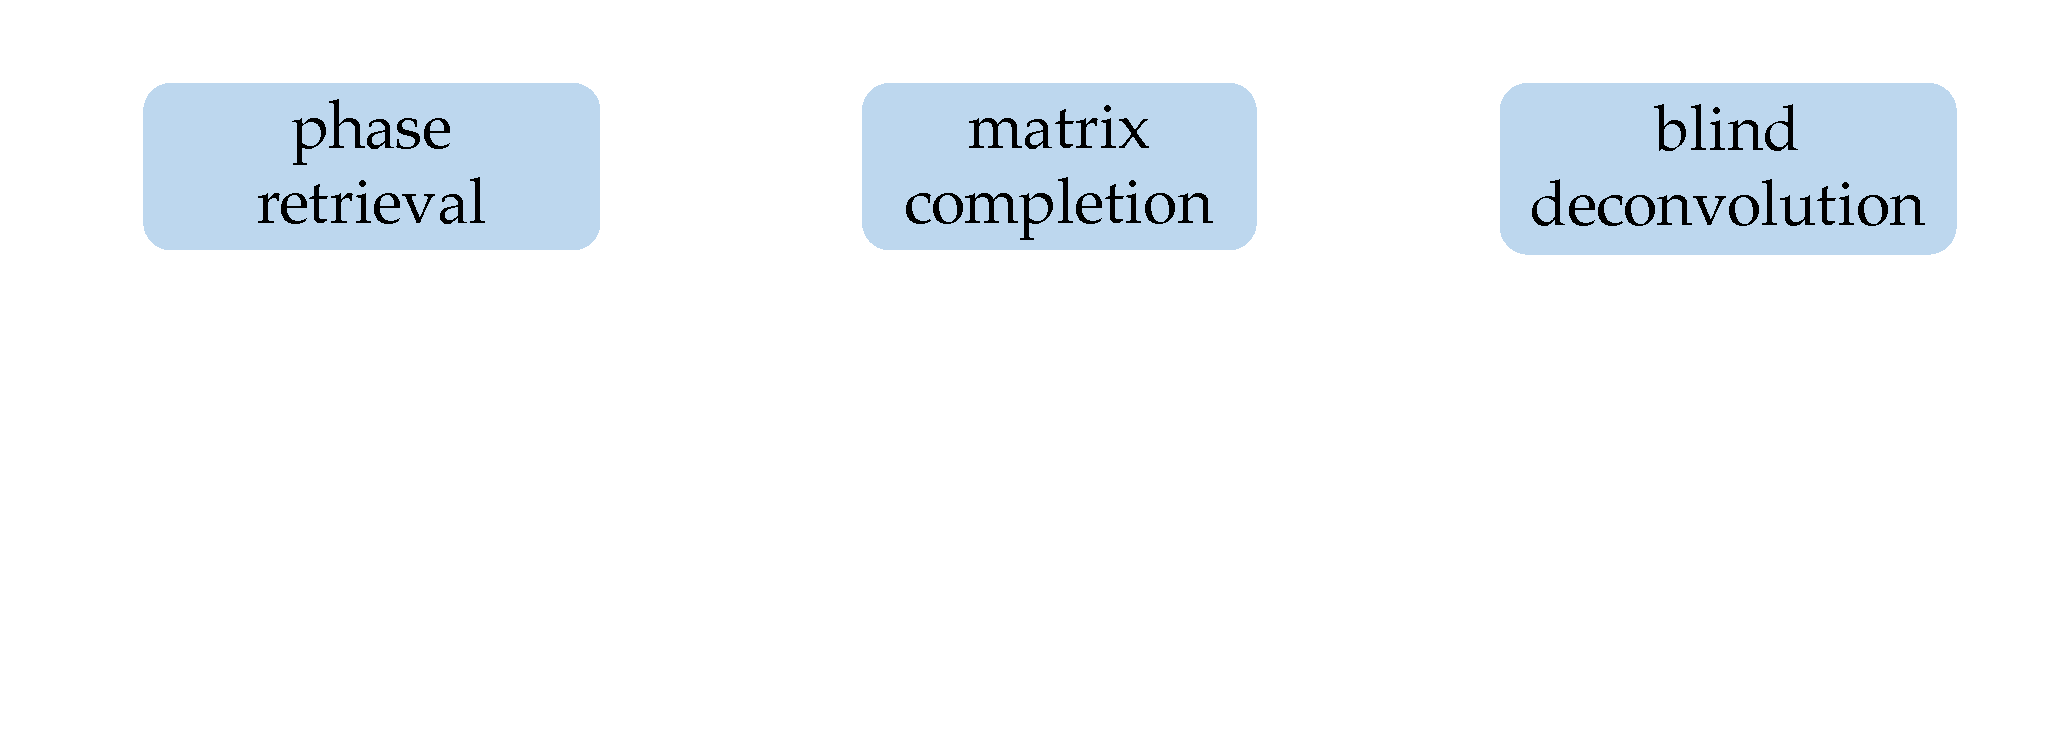
\includegraphics[width=\textwidth]{\yuxinRegFigs/summary.pdf}}\only<2>{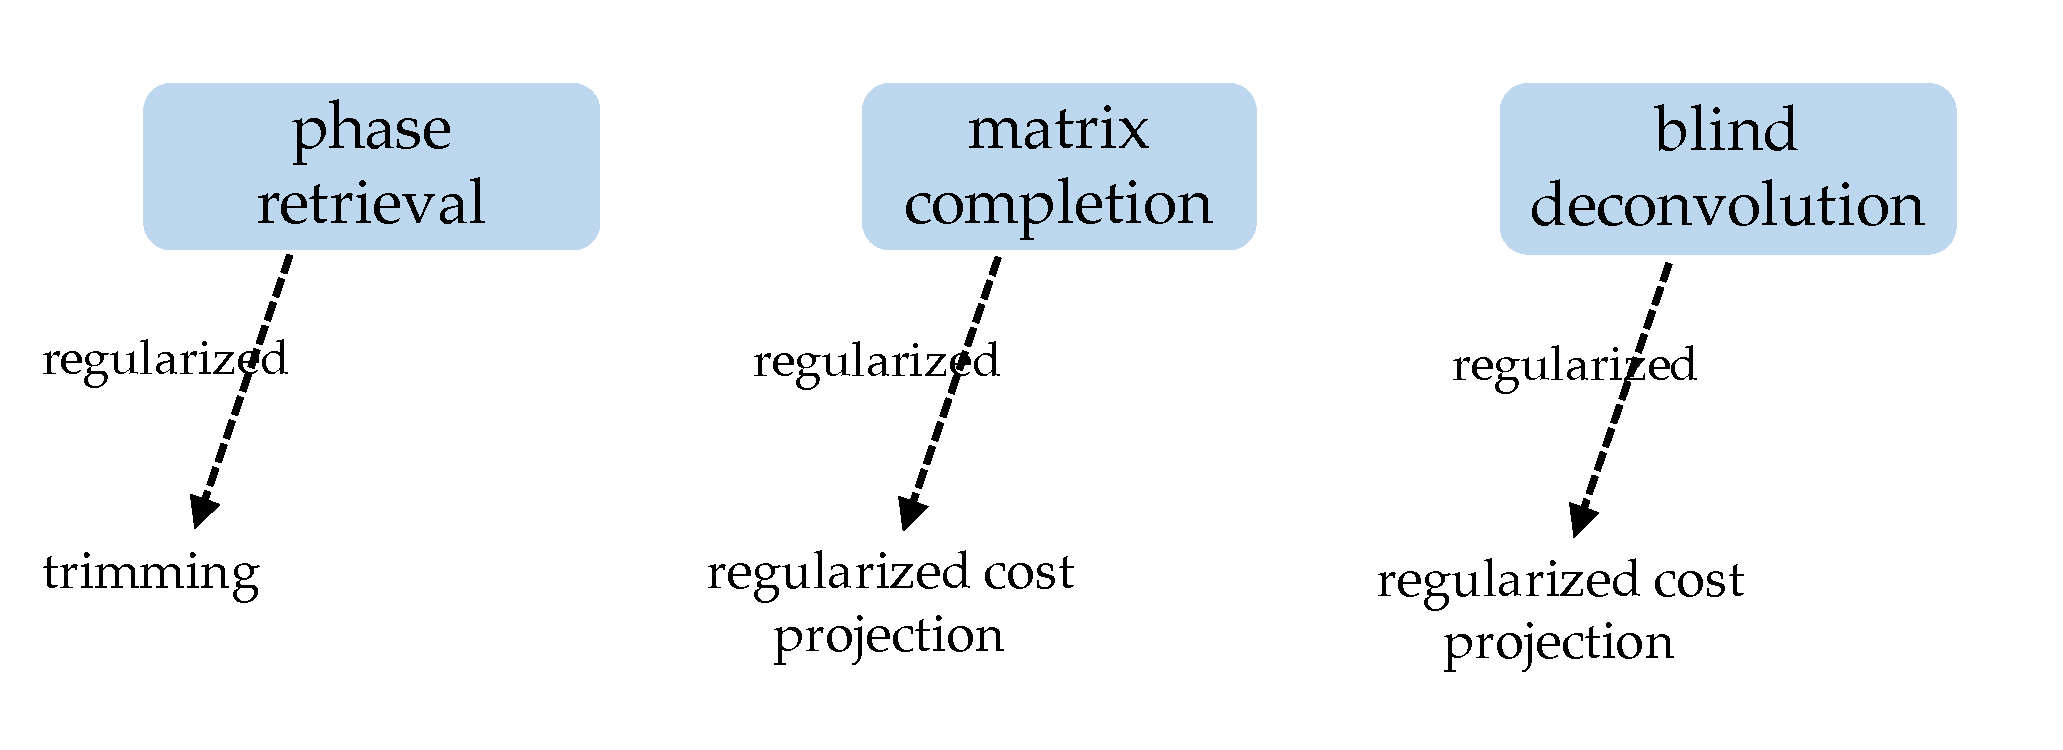
\includegraphics[width=\textwidth]{\yuxinRegFigs/reg_summary.pdf}}\only<3->{\includegraphics[width=\textwidth]{\yuxinRegFigs/reg_unreg_summary.pdf}}
	\end{figure}

\uncover<4->{
{
\setbeamercolor{block body}{bg=babyblueeyes,fg=black}

\begin{varblock}[\textwidth]{}
\begin{center}
	 {\em Are unregularized methods suboptimal for nonconvex estimation? }
\end{center}
\end{varblock}
}
}

\uncover<4->{
\begin{columns}
\begin{column}{0.35\textwidth}
\vspace{-20em}
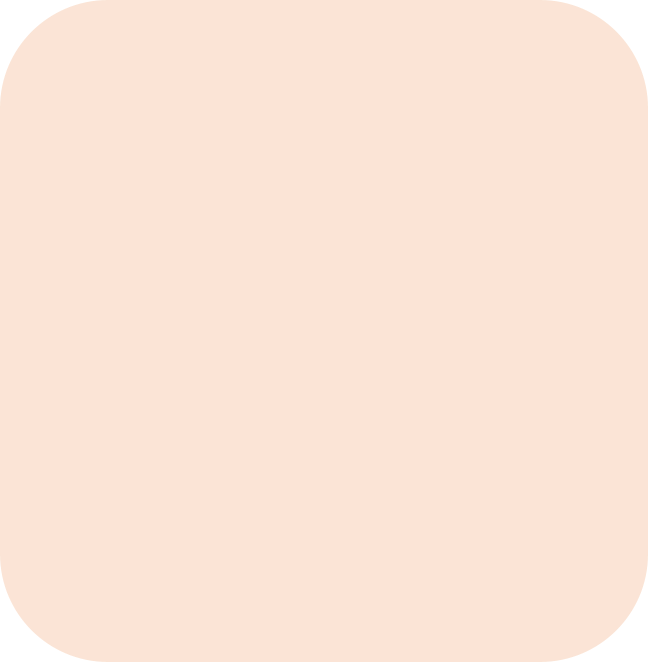
\includegraphics[width=\textwidth]{\yuxinRegFigs/my_frame_orange.png}
\end{column}
\begin{column}{0.6\textwidth}
\end{column}
\end{columns}
}

\end{frame}




\begin{comment}

\begin{frame}
\frametitle{Three representative nonconvex problems}

\vspace{-4em}

\begin{itemize}
	\itemsep1em
  	\item  \only<1->{Phase retrieval / solving random quadratic systems}
		%\only<4->{\alert{Phase retrieval / solving random quadratic systems}}
\begin{align*}
\text{find}\quad  \bm{x}\in\mathbb{R}^{n} \qquad 
\text{s.t.}\quad  \big(\bm{a}_{k}^{\top}\bm{x}\big)^{2}= y_k , ~~ 1\leq k\leq m
\end{align*}
  	%\smallskip

	\pause
 	\item Low-rank matrix completion
\[
\text{find}\text{\quad}\bm{X}\in\mathbb{R}^{n\times r}\qquad\text{s.t.}\quad\bm{e}_{j}^{\top}\bm{X}\bm{X}^{\top}\bm{e}_{k}= M_{j,k},\quad(j,k)\in\Omega
\]
	%\smallskip

	\pause
	\item Blind deconvolution / solving random bilinear systems
\[
\text{find}\text{\quad}\bm{h},\bm{x}\in\mathbb{C}^{n}\qquad\text{s.t.}\quad\bm{b}_{k}^{*}\bm{h}_{k}\bm{x}_{k}^{*}\bm{a}_{k}= y_k,\quad1\leq k\leq m
\]


\end{itemize}


\uncover<4->{
	\vspace{-14.7em}
	%\begin{center}
	%	\includegraphics[width=\textwidth]{\yuxinRegFigs/my_frame.png}
	%\end{center}
{
\setbeamercolor{block body}{bg=babyblueeyes,fg=black}

\begin{varblock}[\textwidth]{}
\begin{itemize}
\item Phase retrieval / solving random quadratic systems
		%\only<4->{\alert{Phase retrieval / solving random quadratic systems}}
\begin{align*}
\text{find}\quad  \bm{x}\in\mathbb{R}^{n} \qquad 
\text{s.t.}\quad  \big(\bm{a}_{k}^{\top}\bm{x}\big)^{2}= y_k , ~~ 1\leq k\leq m
\end{align*}
\end{itemize}
\end{varblock}
}

}


\end{frame}

\end{comment}







\begin{frame}
  \frametitle{Missing phase problem}

Detectors record \alert{intensities} of diffracted rays
  %\alert{$\goto$ phaseless data only!}

  \begin{itemize}
	\item electric field $x(t_1, t_2)$  $\longrightarrow$ Fourier transform $\hat{x}(f_{1},f_{2})$
  \end{itemize}
  \vfill
{\hfill\em\footnotesize Fig credit: Stanford SLAC}
\begin{center}
\includegraphics[width=4cm]{\yuxinRegFigs/microscopy.png} 
\end{center}

{\small
\[
\text{intensity of electrical field: }\big| \hat{x}(f_{1},f_{2}) \big|^2 = \Big|{ \int}x(t_{1},t_{2}) e^{-i2\pi(f_{1}t_{1}+f_{2}t_{2})}\mathrm{d}t_{1}\mathrm{d}t_{2}\Big|^{2}
\]
}
\pause
\vspace{-1em}



{
\setbeamercolor{block body}{bg=babyblueeyes,fg=black}

\begin{varblock}[\textwidth]{}
\begin{center}
   {\bf Phase retrieval:}  recover signal $x(t_{1},t_{2})$ from intensity $| \hat{x}(f_{1},f_{2}) \big|^2$
\end{center}
\end{varblock}
}
	
\end{frame}








\begin{frame}
\frametitle{Solving quadratic systems of equations}

\vspace{-1em}
\begin{figure}
	\centering
	\includegraphics[width=0.95\textwidth]{\yuxinRegFigs/quadratic.pdf}
\end{figure}

Recover $\vct{x}^{\natural} \in \mathbb{R}^n$ from $m$ random quadratic measurements
\begin{eqnarray*}
y_k &= &|\vct{a}_k^\top\vct{x}^{\natural}|^2, \qquad k = 1, \ldots, m  
%\\
%\text{or}\qquad
%\vct{y} &= &|\mtx{A} \vct{x}^{\natural}|^2 \qquad \text{where }|\vct{z}|^2 := [|z_1|^2, \cdots, |z_m|^2]^{\top} 
\end{eqnarray*}

%\medskip
\hfill \textit{Assume w.l.o.g.~}$\|\bm{x}^{\natural}\|_2=1$


%\end{itemize}
\end{frame}






\begin{frame}
\frametitle{Wirtinger flow (Cand\`es, Li, Soltanolkotabi '14)}


Empirical risk minimization
\[
\text{minimize}_{\bm{x}}\quad f(\bm{x})=\frac{1}{4m}\sum_{k=1}^{m}\Big[ \big(\bm{a}_{k}^{\top}\bm{x}\big)^{2}-y_{k} \Big]^{2}
\]


\pause

\vspace{-2em}


\begin{columns}
\begin{column}{0.3\textwidth}

\begin{center}
  \includegraphics[width=1.05\textwidth,angle=-40]{\ProbFigs/GD2.png}
\end{center}

\end{column}



\begin{column}{0.7\textwidth}

\begin{itemize}
\item {\bf Initialization by spectral method}

\bigskip
\bigskip

\item {\bf Gradient iterations:} for $t = 0, 1, \ldots$ 
  \[
  \vct{x}^{t+1}= \vct{x}^t- \eta \, \nabla f(\vct{x}^t)
\]
\end{itemize}

\end{column}
\end{columns}

\end{frame}

%\begin{frame}
%	\frametitle{Existing theory for WF}
%	{
%\setbeamercolor{block body}{bg=babyblueeyes,fg=black}
%
%\begin{varblock}[\textwidth]{}
%{
%{\bf Informal thm (Cand\`es et al '14)}:
%\begin{center}
%  	WF attains $\varepsilon$-accuracy within \alert{$O\big(n\log\frac{1}{\varepsilon}\big)$} iterations \\
%	provided that step size \alert{$\eta \asymp \frac{1}{n}$} and sample size $m \asymp n \log n$
%\end{center}
%}
%\end{varblock}
%}
%\end{frame}


\begin{frame}
\frametitle{Gradient descent theory revisited}



	\begin{figure}
	
		\only<1>{\includegraphics[width=0.5\textwidth]{\ProbFigs/strong_cvx_smoothness1.pdf}}\only<2>{\includegraphics[width=0.5\textwidth]{\ProbFigs/strong_cvx_smoothness2.pdf}}\only<3>{\includegraphics[width=0.5\textwidth]{\ProbFigs/strong_cvx_smoothness3.pdf}}
	\end{figure}



Two standard conditions that enable geometric convergence of GD
\smallskip

	\begin{itemize}
		\itemsep0.3em
		\item<2-> (local) restricted strong convexity (or regularity condition) 

		\item<3-> (local) smoothness

		\vspace{-0.5em}
		\[
			\nabla^2 f( \bm{x} ) \succ \bm{0} \quad \text{and} \quad \text{is well-conditioned} 
		\]
	\end{itemize}


\end{frame}





\begin{frame}
	\frametitle{Gradient descent theory revisited}


	$f$ is said to be $\alpha$-strongly convex and $\beta$-smooth if 
	\[
		\bm{0} ~\preceq~ \alpha \bm{I} ~\preceq~ \nabla^2 f(\bm{x})  ~\preceq~ \beta \bm{I}, \qquad \forall \bm{x}
	\]

\vfill
{
\setbeamercolor{block body}{bg=babyblueeyes,fg=black}

\begin{varblock}[\textwidth]{}
%\begin{center}
  	{\bf $\ell_2$ error contraction:} GD with $\eta = 1/\beta$ obeys
	\vspace{-0.3em}
	\[
		\|\bm{x}^{t+1} -\bm{x}^\natural\|_2 \leq \left(1- \only<1>{\frac{\alpha}{\beta}} 
%		\only<2->{\alert{\frac{\alpha}{\beta}}} 
\right)\|\bm{x}^{t} -\bm{x}^\natural\|_2
	\]
%\end{center}
\end{varblock}
}

%\pause

\begin{itemize}
	\itemsep0.5em
	\item[] \quad
	%\pause
	\item[] \quad
\end{itemize}

\end{frame}



\begin{frame}
	\frametitle{Gradient descent theory revisited}

{
\setbeamercolor{block body}{bg=babyblueeyes,fg=black}

\begin{varblock}[0.7\textwidth]{}
	\vspace{-0.5em}
	\[
		\|\bm{x}^{t+1} -\bm{x}^\natural\|_2 \leq \left(1- \alpha / \beta \right)\|\bm{x}^{t} -\bm{x}^\natural\|_2
	\]
\end{varblock}
}



\begin{center}
	\begin{tabular}{cc}
 	 	
\includegraphics[width=0.04\textwidth]{\ProbFigs/shade.png} 	&  region of local strong convexity + smoothness \tabularnewline
	\end{tabular} 
\end{center}

\vspace{-1em}

\begin{columns}

\begin{column}{0.38\textwidth}
\begin{figure}
	\only<1>{\includegraphics[width=0.9\textwidth]{\ProbFigs/circle0.png}}\only<2>{\includegraphics[width=0.9\textwidth]{\ProbFigs/circle1.png}}\only<3>{\includegraphics[width=0.9\textwidth]{\ProbFigs/circle2.png}}\only<4->{\includegraphics[width=0.9\textwidth]{\ProbFigs/circle3.png}}
\end{figure}
\end{column}


\end{columns}
%\vfill
%\begin{itemize}
%  \itemsep0.5em
%  \item  If this nice region is $\ell_2$ ball and if  we start within this  region, then GD converges fast 
%\end{itemize}


\end{frame}




\begin{frame}
	\frametitle{Gradient descent theory revisited}


	%$f$ is said to be $\lambda$-strongly convex and $\beta$-smooth if 
	\[
		\bm{0} ~\preceq~ \alpha \bm{I} ~\preceq~ \nabla^2 f(\bm{x})  ~\preceq~ \beta \bm{I}, \qquad \forall \bm{x}
	\]


{
\setbeamercolor{block body}{bg=babyblueeyes,fg=black}

\begin{varblock}[\textwidth]{}
%\begin{center}
  	{\bf $\ell_2$ error contraction:} GD with $\eta = 1/{\beta}$ obeys
	\vspace{-0.3em}
	\[
		\|\bm{x}^{t+1} -\bm{x}^\natural\|_2 \leq \left(1- \only<1->{\alert{\frac{\alpha}{\beta}}} \right)\|\bm{x}^{t} -\bm{x}^\natural\|_2
	\]
%\end{center}
\end{varblock}
}



\begin{itemize}
	\itemsep0.5em
	\item Condition number $\alert{\beta / \alpha}$ determines rate of convergence
	\pause
	\item Attains $\varepsilon$-accuracy within $O\big( \alert{ \frac{\beta}{\alpha} } \log\frac{1}{\varepsilon} \big)$ iterations
\end{itemize}

\end{frame}


\begin{frame}
	\frametitle{What does this optimization theory say about WF?}
	

\vspace{-3em}


	\begin{center}
	\begin{equation*}
		\textit{Gaussian designs: } \bm{a}_k ~ \overset{\mathrm{i.i.d.}}{\sim}~ \mathcal{N}(\bm{0}, \bm{I}_n), \quad 1\leq k \leq m
	\end{equation*}
	\end{center}

	\vfill

\uncover<2>{

	{\bf Population level (infinite samples)  } 
	\[
 		\mathbb{E} \big[ \nabla^{2} f(\bm{x}) \big] 
		=
		\underset{\alertb{\textit{locally}\text{ positive definite and well-conditioned}}}{ \underbrace{ 3\left(\left\Vert \bm{x}\right\Vert _{2}^{2}\bm{I} +2\bm{x}\bm{x}^{\top}\right)-\left(\big\Vert \bm{x}^{\natural} \big\Vert _{2}^{2}\bm{I} +2\bm{x}^{\natural}\bm{x}^{\natural\top}\right) }}
	\]

	\vfill	

{
\setbeamercolor{block body}{bg=babyblueeyes,fg=black}

\begin{varblock}[\textwidth]{}
\begin{center}
  	{\bf Consequence:} WF converges within \alert{$O\big(\log\frac{1}{\varepsilon}\big)$} iterations if $m\rightarrow \infty$
\end{center}
\end{varblock}
}
}


\uncover<3->{

\vspace{-11em}

	{\bf Finite-sample level ($m\asymp n\log n$) } 
	\[
 		\nabla^2 f(\bm{x}) ~\succ \bm{0} \quad  
		\uncover<4->{ \underset{ {\alert{\text{condition number}~\asymp~ n}} }{\underbrace{ \text{but ill-conditioned } }}  ~\text{(even locally)} }
	\]

	\vfill	

\uncover<5->
{
\setbeamercolor{block body}{bg=babyblueeyes,fg=black}

\begin{varblock}[\textwidth]{}
\begin{center}
  	{\bf Consequence (Cand\`es et al '14)}:\quad WF attains $\varepsilon$-accuracy within \\ \alert{$O\big(n\log\frac{1}{\varepsilon}\big)$} iterations if $m \asymp n \log n$
\end{center}
\end{varblock}
}

\uncover<6->
{
	\hfill {\em Too slow ... can we accelerate it? }
}

}

\end{frame}



\begin{frame}
\frametitle{One solution: truncated WF (Chen,\,Cand\`es '15)}


Regularize / trim gradient components to accelerate convergence


\vfill
\begin{columns}


\begin{column}{0.6\textwidth}
\centering
\includegraphics[width=\textwidth]{\yuxinTWFfigs/grad_distribution.pdf} \\
\end{column}

\end{columns}

%\medskip

%\pause

%{
%\setbeamercolor{block body}{bg=babyblueeyes,fg=black}
%
%\begin{varblock}[\textwidth]{}
%\begin{center}
%  	With better-controlled search directions, one can proceed much faster
%\end{center}
%\end{varblock}
%}


\end{frame}







\begin{frame}
	\frametitle{But wait a minute ...}

\begin{columns}

\begin{column}{0.92\textwidth}
\begin{itemize}
  \item[] WF converges in $O(n)$ iterations
  \pause

  \vspace{-1em}
  \begin{figure}
	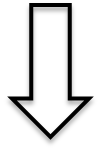
\includegraphics[width=0.05\textwidth,angle=180]{\yuxinRegFigs/arrow_down_3.png} \qquad 
  \end{figure}

  \item[] Step size taken to be \alert{$\eta_t = O(1/n)$}

  \pause
  \vspace{-1em}
  \begin{figure}
	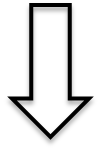
\includegraphics[width=0.05\textwidth,angle=180]{\yuxinRegFigs/arrow_down_3.png} \qquad 
  \end{figure}


  \item[] This choice is suggested by \only<3>{\alert{generic}}\only<4->{\alert{worst-case}} optimization theory

  
  \uncover<5->{
  \vspace{-1em}
  \begin{figure}
	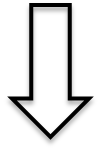
\includegraphics[width=0.05\textwidth,angle=180]{\yuxinRegFigs/arrow_down_3.png}
  \end{figure}


  \item[] Does it capture what really happens? 

  }
\end{itemize}

\end{column}
\end{columns}

\end{frame}




\begin{frame}
	\frametitle{Numerical surprise with $\eta_t  = 0.1$}
\begin{figure}
	\centering
	\includegraphics[width=0.7\textwidth]{\yuxinRegFigs/pr_const_stepsize.pdf}
\end{figure}

{
\setbeamercolor{block body}{bg=babyblueeyes,fg=black}

\begin{varblock}[\textwidth]{}
\begin{center}
  	Vanilla GD (WF) can proceed much more aggressively!
\end{center}
\end{varblock}
}


\end{frame}








\begin{frame}
	\frametitle{A second look at gradient descent theory}



Which region enjoys both strong convexity and smoothness? 

\bigskip
\bigskip

\uncover<1,2>{
\[
	\nabla^2 f(\bm{x})= \frac{1}{m}\sum_{k=1}^m \left[ \alert{3\big(\bm{a}_k^\top \bm{x}\big)^2} -\big(\bm{a}_{k}^{\top}\bm{x}^\natural\big)^2\right]\bm{a}_k\bm{a}_k^\top
\]

}

\bigskip

\uncover<2>{
\begin{itemize}
  \item Not smooth if $\bm{x}$ and $\bm{a}_k$ are too close (coherent)
\end{itemize}
}

\uncover<3->{

\vspace{-11em}

\begin{figure}
	\only<1,2>{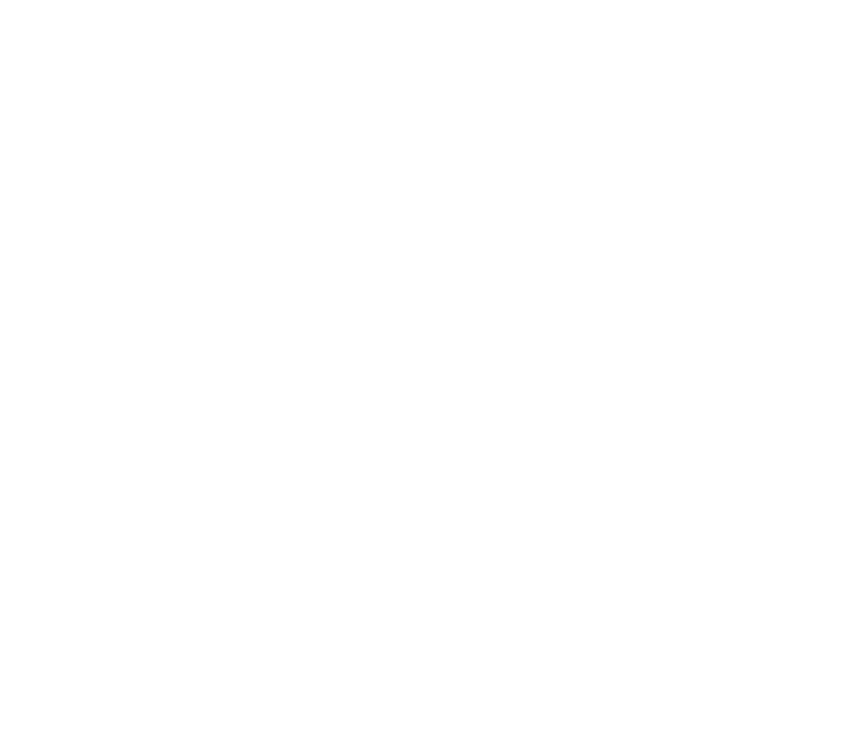
\includegraphics[width=0.6\textwidth]{\yuxinRegFigs/WF_region_0.pdf}}\only<3>{\includegraphics[width=0.6\textwidth]{\yuxinRegFigs/WF_region_3.pdf}}\only<4>{\includegraphics[width=0.6\textwidth]{\yuxinRegFigs/WF_region_2.pdf}}\only<5>{\includegraphics[width=0.6\textwidth]{\yuxinRegFigs/WF_region_1.pdf}}
\end{figure}

\vspace{-2.5em}

\begin{itemize}
  \itemsep0.5em
  \item<3-> $\bm{x}$ is not far away from $\bm{x}^{\natural}$
  \item<4-> $\bm{x}$ is incoherent w.r.t.~sampling vectors \alert{(incoherence region)}
\end{itemize}

}

\end{frame}






\begin{frame}
	\frametitle{A second look at gradient descent theory}


\begin{center}
	\begin{tabular}{cc}
 	 	
\includegraphics[width=0.04\textwidth]{\ProbFigs/shade.png} 	&  region of local strong convexity + smoothness \tabularnewline
	\end{tabular} 
\end{center}

\vspace{-1em}

\begin{columns}

\begin{column}{0.38\textwidth}
\begin{figure}
	\only<1>{\includegraphics[width=0.9\textwidth]{\ProbFigs/circle0.png}}\only<2>{\includegraphics[width=0.9\textwidth]{\ProbFigs/circle1.png}}\only<3>{\includegraphics[width=0.9\textwidth]{\ProbFigs/circle2.png}}\only<4->{\includegraphics[width=0.9\textwidth]{\ProbFigs/circle3.png}}
\end{figure}
\end{column}

\begin{column}{0.42\textwidth}
\begin{figure}
	\only<1-4>{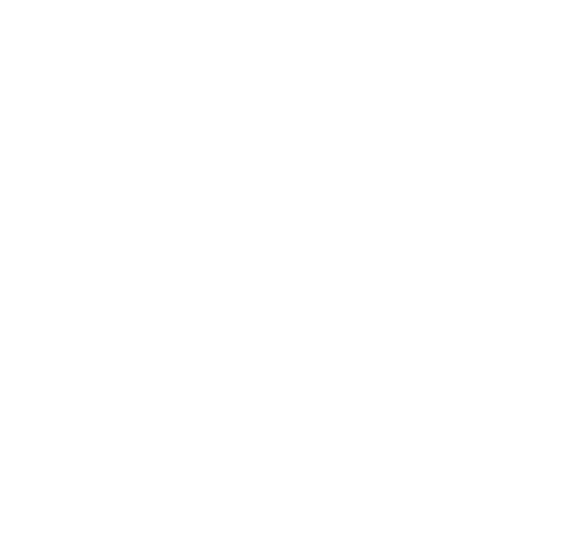
\includegraphics[width=\textwidth]{\ProbFigs/GD_WF_ball5.pdf}}\only<5>{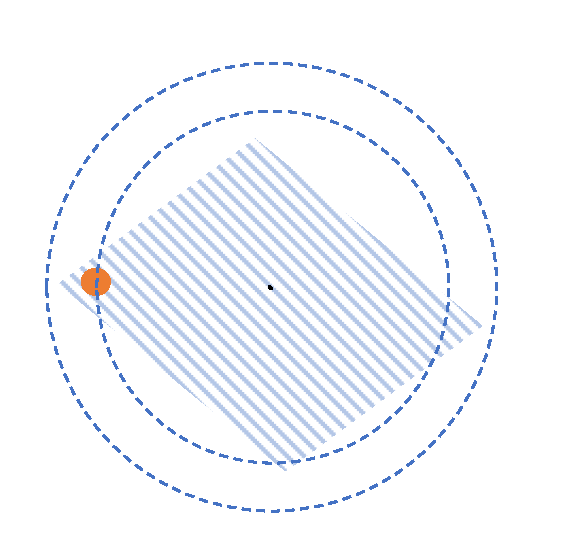
\includegraphics[width=\textwidth]{\ProbFigs/GD_WF_ball4.pdf}}\only<6>{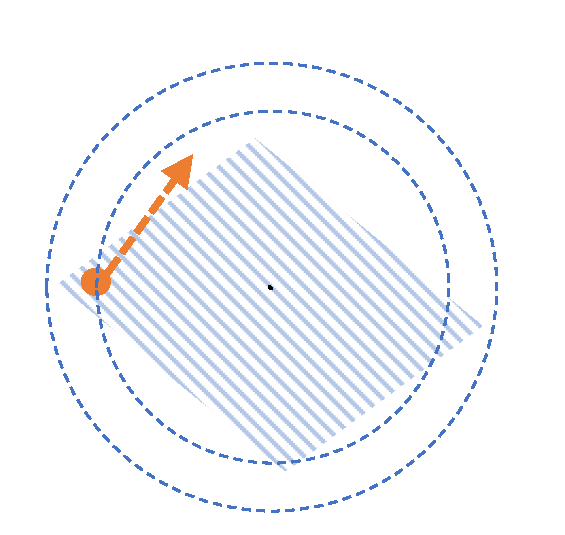
\includegraphics[width=\textwidth]{\ProbFigs/GD_WF_ball3.pdf}}\only<7>{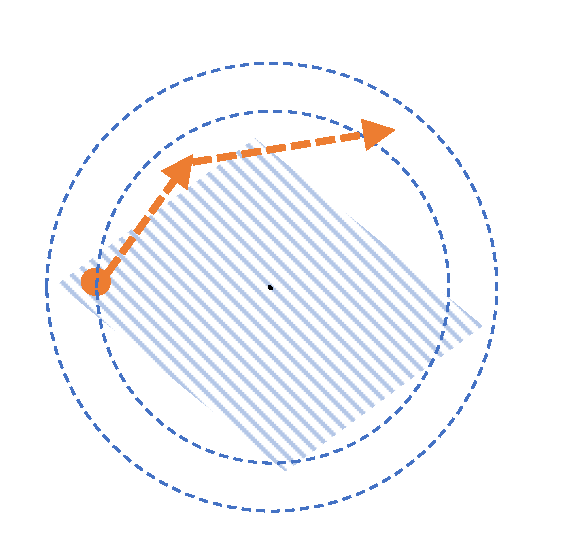
\includegraphics[width=\textwidth]{\ProbFigs/GD_WF_ball2.pdf}}\only<8->{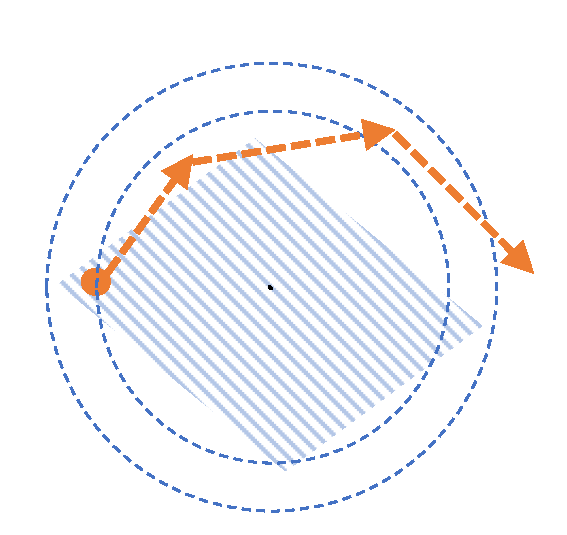
\includegraphics[width=\textwidth]{\ProbFigs/GD_WF_ball1.pdf}}
\end{figure}
\end{column}

\end{columns}
\vfill
\begin{itemize}
  \itemsep0.5em
  \item  Prior theory only ensures that iterates  remain in $\ell_2$ ball but not incoherence region
  \item<9-> {\em Prior theory enforces regularization to promote incoherence}
\end{itemize}


\end{frame}







\begin{frame}
	\frametitle{Our findings: GD is implicitly regularized}


\begin{center}
	\begin{tabular}{cc}
 	 	
\includegraphics[width=0.04\textwidth]{\ProbFigs/shade.png} 	&  region of local strong convexity + smoothness \tabularnewline
	\end{tabular} 
\end{center}

\vspace{-3em}

\begin{columns}


\begin{column}{0.42\textwidth}
\begin{figure}
	\only<1>{\includegraphics[width=\textwidth]{\ProbFigs/GD_WF_ball4_good.pdf}}\only<2>{\includegraphics[width=\textwidth]{\ProbFigs/GD_WF_ball3_good.pdf}}\only<3>{\includegraphics[width=\textwidth]{\ProbFigs/GD_WF_ball2_good.pdf}}\only<4->{\includegraphics[width=\textwidth]{\ProbFigs/GD_WF_ball1_good.pdf}}
\end{figure}

\end{column}

\end{columns}
\vfill


\uncover<5->{

{
\setbeamercolor{block body}{bg=babyblueeyes,fg=black}

\begin{varblock}[0.8 \textwidth]{}
\begin{center}
GD implicitly forces iterates to remain  \alert{incoherent}
\end{center}
\end{varblock}
}
}


\end{frame}





\begin{frame}
	\frametitle{Theoretical guarantees}



\begin{theorem}[Phase retrieval]
Under i.i.d.~Gaussian design, WF achieves 
\begin{itemize}
	\itemsep0.3em
	\item $  \max_k \big| \bm{a}_k^{\top} (\bm{x}^{t}- \bm{x}^{\natural} ) \big | \lesssim \sqrt{\log n} \, \| \bm{x}^{\natural} \|_2$ ~(incoherence)
	\pause
	\item 
$\|\bm{x}^{t}- \bm{x}^\natural\|_2 \lesssim \left(1-\frac{\eta}{2}\right)^{t}\|\bm{x}^\natural\|_{2}$ ~(near-linear convergence)
\end{itemize}
provided that step size $\alert{\eta \asymp \frac{1}{\log n}}$ and
$ \text{sample size}~ m \gtrsim n\log n $.
\end{theorem}



\vfill

\pause

\begin{itemize}
	\itemsep1em
	\item Step size: $\frac{1}{\log n}$ (vs.~$\frac{1}{n}$) 
	\pause
	\item Computational complexity:
	$\frac{n}{\log n}$ times faster than existing theory
\end{itemize}
\end{frame}





\begin{frame}
	\frametitle{Key ingredient: leave-one-out analysis}
For each $1\leq l\leq m$, introduce leave-one-out iterates $\bm{x}^{t,(l)}$ \\ by dropping $l$th measurement
\vfill
\uncover<1->{

\begin{figure}
\centering
\includegraphics[width=0.85\textwidth]{\yuxinRegFigs/pr_leave_one_out.pdf}
\end{figure}
}

\end{frame}


\begin{frame}
	\frametitle{Key ingredient: leave-one-out analysis}

\begin{figure}
\centering
 \only<1>{\includegraphics[width=0.45\textwidth]{\yuxinRegFigs/LOO_sequence.pdf}}\only<2->{\includegraphics[width=0.45\textwidth]{\yuxinRegFigs/LOO_original_sequence.pdf}}
\end{figure}
\begin{itemize}
	\itemsep0.5em
	\item Leave-one-out iterates $\{\bm{x}^{t,(l)}\}$ are independent of $\bm{a}_l$, and are hence {\bf incoherent} w.r.t.~$\bm{a}_l$ with high prob.
	\item<2-> Leave-one-out iterates $\bm{x}^{t,(l)}$ ~$\approx$~ true iterates $\bm{x}^{t}$ 
	\item<3->{
$
\big| \bm{a}_l^{\top} (\bm{x}^{t}- \bm{x}^{\natural} ) \big | \leq \big| \bm{a}_l^{\top} (\bm{x}^{t,(l)}- \bm{x}^{\natural} ) \big | + \big| \bm{a}_l^{\top} (\bm{x}^{t}- \bm{x}^{t,(l)} ) \big |
$
}
\end{itemize}



\end{frame}


\begin{comment}
\begin{frame}[plain]
	\frametitle{}

\vfill 

\centering 
	{\em\large This talk: implicit regularization in nonconvex statistical optimization!}

\vfill

\end{frame}




\begin{frame}
	\frametitle{What does this optimization theory say for WF?}


	Curses of nonconvex formulation:
	\begin{itemize}
		\item \alert{NO} global strong convexity and smoothness
	\end{itemize}
	\vfill
	\pause
	Blessings of randomness:
	\begin{itemize}
		\item w.h.p., $f(\bm{x})$ enjoys \alert{local} strong convexity and smoothness
	\end{itemize}
	\bigskip
\begin{lemma}[Cand\`es,\,Li,\,Soltanolkotabi '14]
$f(\bm{x})$ is $O(1)$-strongly convex and $O(n)$-smooth in the region 
\$
\mathcal{B} = \left\{\bm{x} : \|\bm{x}-\bm{x}^\natural \|_2 \leq \varepsilon \|\bm{x}^\natural\|_2\right\}
\$
% WF yields $\epsilon$-accuracy within \alert{$O\big( n\log\frac{1}{\epsilon}\big)$} iterations 
provided that $ \text{sample size}~ m \gtrsim n\log n $.
\end{lemma}

\end{frame}








\begin{frame}
\frametitle{Performance guarantee of WF}

%\vspace{-1em}
%\hfill {\small{\em Cand\`es, Li and Soltanolkotabi ('14)}} \\
%\hfill {\small{\em Soltanolkotabi ('14)}}
\begin{theorem}[Cand\`es, Li, Soltanolkotabi '14]
Under i.i.d.~Gaussian design, WF achieves
\[
  \|\vct{x}^t- \vct{x}^\natural\|_2 \lesssim \left( 1 - \frac{\eta}{4} \right)^{t/2} \|\vct{x}^\natural \|_2, 
\]

% WF yields $\epsilon$-accuracy within \alert{$O\big( n\log\frac{1}{\epsilon}\big)$} iterations 
provided that step size $\alert{\eta \lesssim \frac{1}{n}}$ and
$ \text{sample size}~ m \gtrsim n\log n $.
\end{theorem}
\begin{itemize}
	\item Conservative step size: $\eta \lesssim \frac{1}{n}$
	\item Computational cost: $O\left(mn^2 \log \frac{1}{\varepsilon}\right)$
\end{itemize}
$O\left(\underbrace{mn}_{\text{cost per iter}} \cdot \underbrace{n}_{\text{condition number}} \log \frac{1}{\varepsilon}\right)$
\end{frame}








\begin{frame}
	\frametitle{Implicit regularization improves smoothness}
\begin{lemma}[Local strong convexity and smoothness]
$f(\bm{x})$ is $O(1)$-strongly convex and \alert{$O(\log n)$}-smooth in the region 
\$
\mathcal{B}^{\text{inc}} = \left\{\bm{x} : \|\bm{x}-\bm{x}^\natural\|_2 \leq \varepsilon \|\bm{x}^\natural \|_2\right\} \cap \left\{\bm{x} : \max_{1\leq k \leq m}|\bm{a}_k^\top \bm{x}| \leq \sqrt{\log n}\|\bm{x}^\natural\|_2\right\}
\$
% WF yields $\epsilon$-accuracy within \alert{$O\big( n\log\frac{1}{\epsilon}\big)$} iterations 
provided that $ \text{sample size}~ m \gtrsim n\log n $.
\end{lemma}


\end{frame}

\end{comment}


%\begin{frame}
%	\frametitle{General recipe: a leave-one-out analysis}
%	
%	\begin{itemize}\itemsep0.5em
%		\item[{\bf Step 1:}] identify the region of incoherence
%and characterize restricted strong convexity and smoothness of $f$;
%		\item[{\bf Step 2:}] introduce leave-one-out sequences $\{\bm{x}^{t,(l)}\}$
%for each $l$; 
%		\item[{\bf Step 3:}] establish the incoherence condition for $\{\bm{x}^t\}$ via induction. 
%
%\end{itemize}
%	
%\end{frame}


\begin{frame}[plain]
	\frametitle{}

\vfill 

\centering 
	{\em\Large This recipe is quite general}

\vfill

\end{frame}




\begin{frame}
\frametitle{Low-rank matrix completion}



\begin{columns}
\begin{column}{0.5\textwidth}
\[
 \begin{bmatrix}
   {\color{blue} \checkmark} & {\color{red} ?} &{\color{red} ?}  & {\color{red} ?} & {\color{blue} \checkmark} & {\color{red} ?} \\
   {\color{red} ?} & {\color{red} ?} & {\color{blue} \checkmark} & {\color{blue} \checkmark} & {\color{red} ?} & {\color{red} ?} \\
   {\color{blue} \checkmark} & {\color{red} ?} & {\color{red} ?} & {\color{blue} \checkmark} & {\color{red} ?} & {\color{red} ?} \\
   {\color{red} ?} & {\color{red} ?} & {\color{blue} \checkmark}  & {\color{red} ?} &{\color{red} ?}  & {\color{blue} \checkmark} \\
   {\color{blue} \checkmark}  &  {\color{red} ?} & {\color{red} ?} & {\color{red} ?}  & {\color{red} ?} & {\color{red} ?} \\
   {\color{red} ?} & {\color{blue} \checkmark} &{\color{red} ?}  & {\color{red} ?} & {\color{blue} \checkmark} & {\color{red} ?} \\
   {\color{red} ?}  &{\color{red} ?} & {\color{blue} \checkmark} &
   {\color{blue} \checkmark} & {\color{red} ?} & {\color{red} ?}
\end{bmatrix}
\]
\end{column}

\begin{column}{0.5\textwidth}  
\begin{center}
\includegraphics[width=0.9\textwidth]{\yuxinRegFigs/NetflixMahdi} \\
\hfill {\footnotesize\em Fig.~credit: Cand\`es ~~}
\end{center}
\end{column}

\end{columns}

\bigskip
%\begin{itemize}
%\item 

Given partial samples $\Omega$ of a {\em low-rank} matrix $\bm{M}$, fill in missing entries 
%\item Seems hopeless

%\end{itemize}

\end{frame}



\begin{frame}
	\frametitle{Prior art}

\[
\text{minimize}_{\bm{X}}\quad f(\bm{X})=\sum_{(j,k)\in\Omega}\Big(\bm{e}_{j}^{\top}\bm{X}\bm{X}^{\top}\bm{e}_{k}-M_{j,k} \big)^{2}
\]

\vfill

\pause
Existing theory on gradient descent requires  
\medskip
\begin{itemize}
  \itemsep1em
  \pause
  \item regularized loss  (solve $\min_{\bm{X}}~f(\bm{X}) \alert{+R(\bm{X})}$ instead)
  \begin{itemize}
	\item e.g.~Keshavan,\,Montanari,\,Oh '10, Sun,\,Luo '14, Ge,\,Lee,\,Ma '16
  \end{itemize}

  \pause
  \item projection onto set of incoherent matrices 
  \begin{itemize}
	\item e.g.~Chen,\,Wainwright '15, Zheng,\,Lafferty '16

  \end{itemize}
\end{itemize}

\end{frame}




\begin{frame}
	\frametitle{Theoretical guarantees}
	\begin{theorem}[Matrix completion]
Suppose $\bm{M}$ is rank-$r$, incoherent and well-conditioned.  \alert{Vanilla gradient descent} (with spectral initialization) achieves $\varepsilon$ accuracy
%\[
% \left\Vert \bm{X}^{t}\bm{R}^{t}-\bm{X}^{\natural}\right\Vert _{\mathrm{F}}\leq\left\{ C_{1}\rho^{t}\mu r\frac{1}{\sqrt{np}}+C_{2}\frac{\sigma}{\sigma_{\min}}\sqrt{\frac{n}{p}}\right\} \left\Vert \bm{X}^{\natural}\right\Vert _{\mathrm{F}},
%\] 
\begin{itemize}
	\item in $O\big(\log\frac{1}{\varepsilon}\big)$ iterations \uncover<2->{w.r.t.~\alertb{$\|\cdot\|_{\mathrm{F}}$, $\|\cdot\|$,} and \alertb{$\underset{\text{incoherence}}{\underbrace{\|\cdot\|_{2,\infty}}}$ }}
\end{itemize}
if step size $\eta \lesssim 1/\sigma_{\max}(\bm{M})$ and $\text{sample size} \gtrsim n r^3 \log^3 n $
\end{theorem}

\medskip

\begin{itemize}
	\itemsep0.5em
	%\item<3-> Regularization-free
	\item<3-> {\em Byproduct: vanilla GD controls {\bf\em entrywise error} \\--- errors are spread out across all entries }
\end{itemize}
\end{frame}



\begin{comment}
\begin{frame}
	\frametitle{Byproduct: entrywise error}
	\begin{theorem}[Matrix completion entrywise error]
Suppose $\bm{M}^\natural$ is $\mu$-incoherent, \alert{plain gradient descent} achieves
%\[
% \left\Vert \bm{X}^{t}\bm{R}^{t}-\bm{X}^{\natural}\right\Vert _{2,\infty}\leq\left\{ C_{1}\rho^{t}\mu r\sqrt{\frac{\log n}{np}}+C_{2}\frac{\sigma}{\sigma_{\min}}\sqrt{\frac{n\log n}{p}}\right\} \left\Vert \bm{X}^{\natural}\right\Vert _{2,\infty},
%\] 
\begin{itemize}
	\item exponential decay in entrywise error
\end{itemize}
provided that $\eta \lesssim \frac{1}{\sigma_{\max}}$ and
$ \text{sample size}~ n^2 p \gtrsim \mu^3 r^3 n\log^3 n $.
\end{theorem}
Implication: 
\begin{align*}
	\left\Vert \bm{X}^{t}\bm{X}^{t\top}-\bm{M}^{\natural}\right\Vert _{\infty}\lesssim\left(\rho^{t}\mu r\sqrt{\frac{\log n}{np}}+\frac{\sigma}{\sigma_{\min}}\sqrt{\frac{n\log n}{p}}\right)\left\Vert \bm{M}^{\natural}\right\Vert _{\infty}
\end{align*}
\end{frame}
\end{comment}



\begin{frame}
	\frametitle{Blind deconvolution}
	\begin{columns}

\begin{column}{0.6\textwidth}
\begin{figure}
	{\includegraphics[width=0.9\textwidth]{\ProbFigs/image_deblurring.jpg}}
	\hfill {\footnotesize\em Fig.~credit:  Romberg~~}
\end{figure}
\end{column}

\begin{column}{0.35\textwidth}
\begin{figure}
	{\includegraphics[width=0.9\textwidth]{\ProbFigs/multipath.jpg}}
	\hfill {\footnotesize\em Fig.~credit:  EngineeringsALL~~}
\end{figure}
\end{column}
\end{columns}
\vfill

Reconstruct two signals from their convolution; equivalently,

\[
\text{find}\text{\quad}\bm{h},\bm{x}\in\mathbb{C}^{n}\qquad\text{s.t.}\quad\bm{b}_{k}^{*}\bm{h}\bm{x}^{*}\bm{a}_{k}= y_k,\quad1\leq k\leq m
\]

\end{frame}

\begin{frame}
	\frametitle{Prior art}

\[
	\text{minimize}_{\bm{x},\bm{h}}\quad f(\bm{x},\bm{h})=\sum_{k=1}^{m}\left|\bm{b}_{k}^{*}\left(\bm{h}\bm{x}^{*}-\bm{h}^{\natural}\bm{x}^{\natural*}\right)\bm{a}_{k}\right|^{2}
\]


\[
	\bm{a}_k ~\overset{\mathrm{i.i.d.}}{\sim}~ \mathcal{N}(\bm{0},\bm{I}) \qquad \text{and} \qquad \{\bm{b}_k\}: \text{ partial Fourier basis}
\]


\vfill

\pause
Existing theory on gradient descent requires  
\medskip
\begin{itemize}
  \itemsep1em
  \item regularized loss + projection 
  \begin{itemize}
        \itemsep0.5em
	\item e.g.~Li,\,Ling,\,Strohmer,\,Wei '16,  Huang,\,Hand '17,  Ling,\,Strohmer '17
	\pause
	\item requires $m$ iterations even with regularization
  \end{itemize}
\end{itemize}

\end{frame}


\begin{frame}
	\frametitle{Theoretical guarantees}
	\begin{theorem}[Blind deconvolution]
Suppose $\bm{h}^\natural$ is incoherent w.r.t.~$\{\bm{b}_k\}$. \alert{Vanilla gradient descent} (with spectral initialization) achieves $\varepsilon$ accuracy in $O\big(\log \frac{1}{\varepsilon}\big)$ iterations, 
%\begin{itemize}
%	\item geometric convergence
%\end{itemize}
provided that step size $\eta \lesssim 1$ and
$ \text{sample size}~ m \gtrsim n \mathrm{poly}\log(m)$.
\end{theorem}

\vfill

\begin{itemize}
	\itemsep0.5em
	\item Regularization-free
	\item Converges in $O\big(\log \frac{1}{\varepsilon}\big)$ iterations (vs.~$O\big(m\log \frac{1}{\varepsilon}\big)$ iterations in prior theory)
\end{itemize}
\end{frame}



\begin{frame}
	\frametitle{Incoherence region in high dimensions}

\begin{center}
\begin{tabular}{cc}
 \includegraphics[width=0.4\textwidth]{\yuxinRegFigs/GD_converge_2D.pdf}& \includegraphics[width=0.4\textwidth]{\yuxinRegFigs/GD_converge_highD.pdf}\tabularnewline
 2-dimensional & $\underset{\alertb{\text{incoherence region is vanishingly small}}}{\underbrace{\text{high-dimensional (mental representation)}}}$ \tabularnewline
\end{tabular}
%
\end{center}
\end{frame}



\begin{frame}[plain]
\frametitle{Complicated dependencies across iterations}

\begin{itemize}
  \item Several prior sample-splitting approaches: require \alert{fresh samples} at each iteration; not what  we actually run in practice 
\end{itemize}
  \begin{center}
     \includegraphics[width=0.65\textwidth]{\yuxinTWFfigs/path_fresh.pdf} 
  \end{center}


\uncover<2>{
\begin{itemize}
     \item  {\bf This work:} reuses all samples in all iterations
\end{itemize}
  \begin{center}
     \includegraphics[width=0.65\textwidth]{\yuxinTWFfigs/path_dependent.pdf} 
  \end{center}
}

\end{frame}



\begin{frame}
	\frametitle{Summary}

	\begin{itemize}
		\itemsep0.5em
		%\item {\bf Blessings of randomness:} nonconvex statistical optimization may not be that scary

		%\pause
		\item {\bf Implicit regularization:} vanilla gradient descent automatically forces iterates to stay {\em incoherent}

		\pause
		\item Enable error controls in a much stronger sense (e.g.~{\em entrywise error control})
		%\item Lots of applications: phase retrieval, matrix completion, blind deconvolution, mixture models, etc.
	\end{itemize}

\vfill

	{\footnotesize \textbf{Paper}: \\ \vspace{1em} ``{Implicit regularization in nonconvex statistical estimation:  Gradient descent converges linearly for phase retrieval, matrix completion, and blind deconvolution}'', Cong Ma, Kaizheng Wang, Yuejie Chi, Yuxin Chen, arXiv:1711.10467}



\end{frame}


\end{document}

